\begin{figure}
	\centering%
	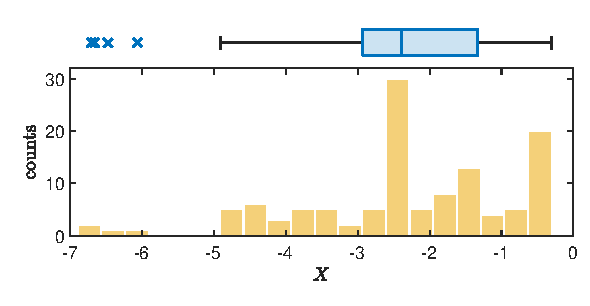
\includegraphics[width=\hsize]{\ROOTPATH/fig1.pdf}
	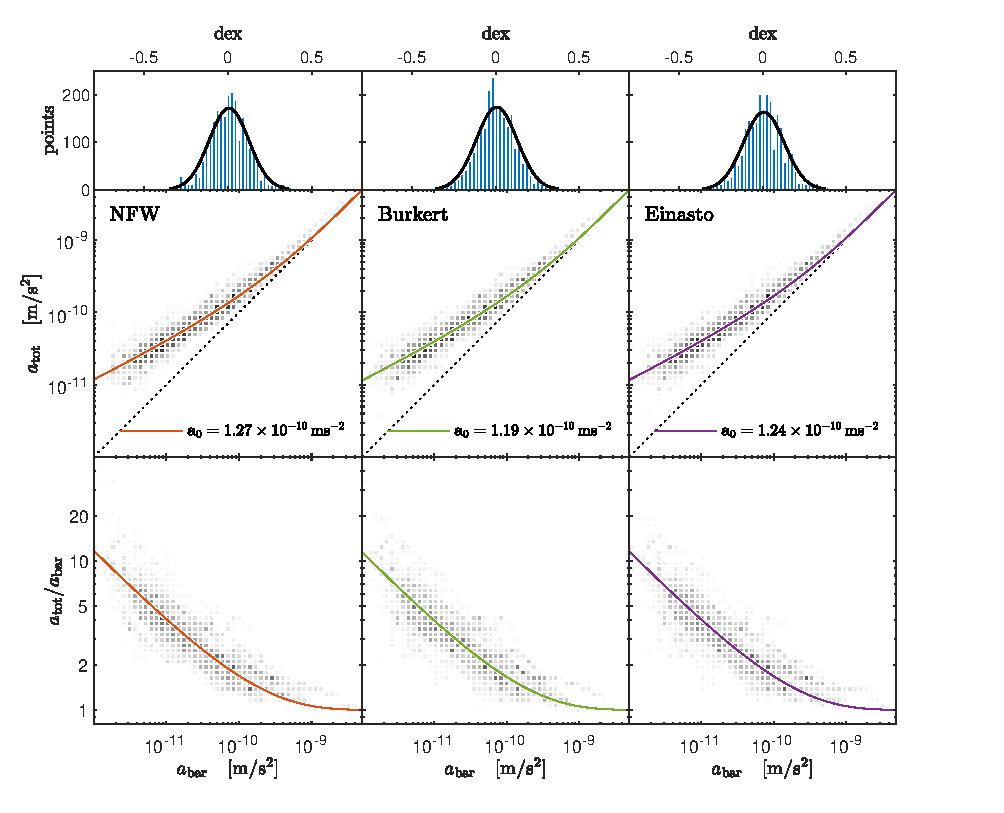
\includegraphics[width=\hsize]{\ROOTPATH/fig2.pdf}
	\caption{Distribution of the best-fit parameters for the DC14 model. Above the histogram a boxplot is shown with a median value at $X \approx -2.4$. The mean value is very close to the median value. The corresponding values for $\alpha$, $\beta$ and $\gamma$ are calculated from the best-fitted $X$ value following \cref{eqn:dc14:alpha,eqn:dc14:beta,eqn:dc14:gamma}.}%
	\label{fig:parameter-distribution:dc14}%
\end{figure}